\subsection{TAXII}

\textit{Trusted Automated eXchange of Indicator Information} (TAXII) es un conjunto de especificaciones técnicas y de documentación para permitir el intercambio de información procesable entre organizaciones.
Tiene como objetivo extender la capacidad de compartir indicadores, 
siendo dichos intercambios robustos, seguros y de gran volumen de datos. A su 
vez, los datos intercambiados deberían ser mas expresivos que en la actualidad.\\

Con TAXII no se busca crear una comunidad para compartir, sino que se le da a 
las organizaciones una herramienta que facilite el intercambio entre ellas. 
TAXII mejora las deficiencias existentes en el intercambio de información de seguridad, esto lo hace dando especificaciones abiertas y comunes para realizar dicho intercambio. También se provee un 
conjunto de capacidades como encriptación, autenticación, direccionamiento, 
alertas y pedidos entre sistemas.\\

Para realizar los intercambios de información se definen protocolos y formatos de datos que 
permiten intercambiar información de forma segura. Ha sido diseñado para permitir la
interoperabilidad de diferentes soluciones en lugar de ligarse a una tecnología o producto en particular.
Además, se busca incentivar a los proveedores de tecnología a incorporar soporte para las especificaciones
de TAXII en sus productos. La información intercambiada 
ayuda a detectar, prevenir y mitigar amenazas informáticas en tiempo real. 

Es importante recalcar que en TAXII no se buscan definir los aspectos no técnicos del intercambio de información, un ejemplo de esto es los acuerdos de confianza que se dan entre las organizaciones. En su lugar, permite a las organizaciones mejorar el 
contexto en el que se encuentran respecto a las nuevas amenazas y además 
compartir la información que ellos elijan con las organizaciones que deseen de 
forma simple y rápida aprovechando las relaciones y sistemas existentes.\\

Durante el desarrollo de STIX y TAXII, MITRE buscó consenso y participación de la comunidad. 
TAXII permite el intercambio de información sobre amenazas de forma eficiente y 
comprensiva por medio de \emph{automatización} y \emph{articulación} de un 
modelo detallado de información. Para lograr esto, se utiliza una representación 
estándar de información de amenazas y un framework para soportar el intercambio 
de datos. La representación por medio de STIX permite la representación de un conjunto amplio de información de seguridad. Se le da la libertad a los proveedores de determinar como sus 
productos producen, consumen o toman ventaja de los flujos de información 
especificados por TAXII.\\

 
\begin{figure}[ht!]
  \centering
    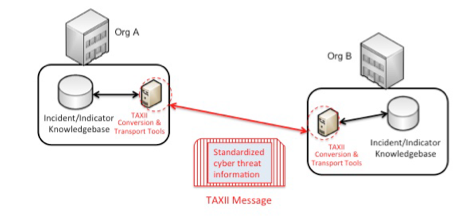
\includegraphics[scale=0.80]{./images/TAXIIArchitecture1.png}
    \caption{Arquitectura de TAXII \protect\cite{b1}}
    \label{fig.diagramabloques}
\end{figure}

TAXII utiliza protocolos y especificaciones existentes siempre que 
es posible, por ejemplo, durante la primera especificación se utilizaron los protocolos HTTP/HTTPS para el intercambio de información entre organizaciones. Esto ayuda a reducir costos de impementación y facilita la adopción de TAXII por parte de organizaciones ya establecidas.\\

Las motivaciones para tener una mejor solución que permita intercambiar 
información lleva a que en el diseño de TAXII se hayan planteado los siguientes 
objetivos:
 \begin{itemize}
   \item Permitir el intercambio seguro y rápido de información referente a 
   amenazas entre comunidades de defensores de seguridad.
   \item Lograr un estándar para permitir compartir indicadores entre organizaciones.
   \item Extender el intercambio de indicadores para permitir intercambios 
   seguros, robustos y de gran volumen que tengan una expresividad mayor a la 
   actual.
   \item Soportar un amplio número de casos de uso y prácticas comunes a las 
   comunidades.
   \item Siempre que existan estándares adecuados que solucionen una parte del problema, TAXII propone que estos sean utilizados.
   \item Llegar a una adopción por parte de organizaciones internacionales de 
   estándares.
 \end{itemize}

Para automatizar el intercambio de información, es necesario especificar como 
ésta es compartida. Para lograr esto, TAXII define especificaciones técnicas y 
documentación de soporte. En particular, las especificaciones de TAXII definen 
un conjunto de capacidades necesarias para el transporte exitoso de mensajes. 
Los mensajes TAXII llevan datos de amenazas informáticas representados por medio de STIX. El conjunto completo de los mensajes incluyen mensajes con datos y 
de control.\\

\subsubsection{TAXII Toolkit}\ \\

Es provisto para soportar la adopción de TAXII y asistir en el desarrollo de 
capacidades compatibles. El \textit{toolkit} provee una colección de implementaciones de 
referencia, un conjunto de herramientas y una colección de librerías e 
interfaces.\\

TAXII está definido por múltiples especificaciones relacionadas. Esta sección 
describe las especificaciones definidas en TAXII.

\begin{itemize}
  \item \underline{Especificación de servicios}: Provee los requerimientos por los cuales se 
  definen los servicios e intercambios de TAXII. No provee detalles respecto al 
  formato de los datos o como los mensajes TAXII son transportados por la red. 
  Dichos detalles y requerimientos pueden ser encontrados en la especificación 
  de los protocolos de enlace y en la especificación de mensajes de enlace.
 \item \underline{Especificación de protocolos de enlace}: Define los requerimientos para 
 transportar mensajes TAXII por la red. Puede haber varias especificaciones 
 creadas para TAXII. Cada especificación define requerimientos para el 
 transporte de mensajes TAXII utilizando protocolos de red y se proveen 
 requerimientos respecto a como los servicios TAXII son soportados por los 
 protocolos de red.
 \item \underline{Especificación de mensajes de enlace}: Se definen requerimientos para 
 representar mensajes TAXII en un formato particular. Puede haber múltiples 
 especificaciones para dichos mensajes. Se provee información detallada sobre 
 como las especificaciones definidas en la especificación de servicios son 
 expresadas en los mensajes.
\end{itemize}

Para dar flexibilidad en el proceso evolutivo de TAXII, se han separado las 
especificaciones de servicios, de los protocolos de enlace y de los mensajes de 
enlace.
Debido a que las organizaciones generalmente tienen restricciones 
respecto a los protocolos que soportan, TAXII busca no ligarse a un único 
protocolo que excluya a una parte de la comunidad. Cuando se ve que la comunidad 
expresa interés en un nuevo protocolo o tipo de mensaje, TAXII puede dar soporte 
a los nuevos protocolos o tipos de mensajes sin cambiar los componentes centrales.\\

Dos grupos que usen el mismo protocolo de red y formato de mensajes serán 
capaces de intercambios de información estructurada de forma automática. Las 
políticas de intercambio de los participantes pueden limitar estos intercambios 
si es necesario, pero el uso de servicios compatibles con TAXII asegura que se 
puede intercambiar cualquier información con los mecanismos definidos por TAXII. 
Los grupos que usen diferentes protocolos o formatos de mensajes no serán 
capaces de comunicarse directamente, pero como están utilizando mensajes y 
servicios en el núcleo de las comunicaciones de sus comunidades significa que es 
posible establecer caminos para que ocurra la interacción.

\subsubsection{Especificación de Servicios}\ \\

Esta especificación provee normativas respecto a los servicios, mensajes e 
intercambios de mensajes en TAXII. No provee detalles respecto a como los 
mensajes son transportados, dejando eso a la especificación de los protocolos de 
enlace. Se da información respecto a los datos presentes en los mensajes TAXII y 
no a como los mensajes son expresados.\\

Una unidad funcional es una componente de TAXII con un rol bien definido dentro del protocolo. 
Las unidades funcionales de TAXII representan conjuntos discretos de actividades 
requeridas para soportar TAXII.

\begin{itemize}
  \item \underline{Arquitectura TAXII}: Cubre los aspectos de las unidades funcionales de la 
  infraestructura de productor o consumidor que provee o utiliza servicios 
  TAXII. Una arquitectura TAXII incluye una TTA, un TMH y un backend TAXII, cada una de estas componentes será descripta a continuación.
  \item \underline{TAXII Transfer Agent} (TTA): Es una unidad funcional conectada a la red 
  que envía o recibe mensajes TAXII. Una TTA interactúa con otras TTAs por medio 
  de la red y maneja los requerimientos de las distintas especificaciones de 
  los protocolos de enlace. Una TTA provee un mensaje TAXII a un \textit{TAXII Message 
  Handler} permitiendo que éste último sea independiente del protocolo de red 
  utilizado. De la misma forma, el TTA puede ser independiente del contenido de 
  los mensajes TAXII, dejando el manejo de la información al \textit{TAXII Message 
  Handler}.
  \item \underline{TAXII Messsage Handler} (TMH): Es una unidad funcional que produce y 
  consume mensajes TAXII. EL TMH es responsable de parsear y construir mensajes 
  con el formato especificado en uno o más TAXII \textit{Message Binding Specifications}. 
  Un TMH interactúa con un TTA, el cual maneja los detalles necesarios para 
  transmitir mensajes por la red. El Backend TAXII interactúa con el TMH para 
  convertir su contenido en mensajes TAXII y llevar a cabo actividades basadas 
  en los mensajes TAXII que son recibidos por el TMH.
  \item \underline{Backend TAXII}: Las especificaciones de TAXII no proveen requerimientos sobre como son 
  implementadas las capacidades en un backend más allá de como debe interactuar 
  con el TMH. Las organizaciones o implementadores pueden decidir que 
  capacidades implementar según los servicios TAXII que deseen soportar o según 
  como quieran dar ese soporte.
  \end{itemize}

Lo expresado anteriormente se puede ver en la figura \ref{fig.unidades_funcionales}.

\begin{figure}[ht!]
  \centering
    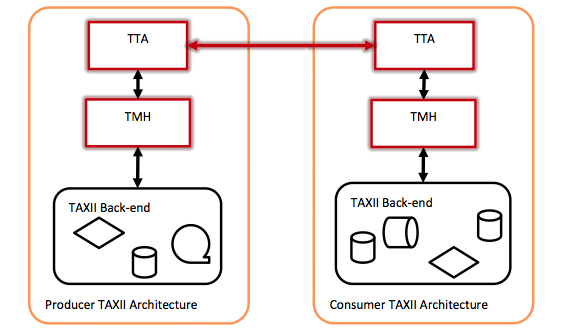
\includegraphics[width=150mm]{./images/TAXIIArchitecture.png}
    \caption{Unidades funcionales de TAXII \protect\cite{b1}}
    \label{fig.unidades_funcionales}
\end{figure}

\newpage
\subsubsection{Capacidades}\ \\

TAXII provee capacidades específicas para aquellos que desean compartir 
información de amenazas cibernéticas. Las capacidades TAXII son el nivel más 
alto en el cual se pueden expresar las acciones de TAXII. Hay tres capacidades 
que soporta la actual versión de TAXII, estas son: \textit{push messaging}, \textit{pull 
messaging} y \textit{discovery}.\\

En \textit{\textbf{push messaging}} la información puede ser enviada de un productor a un 
consumidor. Esto puede reflejar una relación pre-existente entre el productor y 
el consumidor en la que el consumidor ha pedido que se le envíen datos desde el 
productor. También puede usarse en caso de que el consumidor desee aceptar 
contribuciones de cualquier productor, y estos le envíen datos en cualquier 
momento.\\

\textit{\textbf{Pull messaging}} permite a un consumidor requerir información de un productor. 
Esto no solo le permite al consumidor el control sobre el momento en el que 
recibe los datos sino que también le permite hacerlo sin tener que aceptar 
conexiones entrantes. Así como en \textit{push messaging}, el productor y consumidor 
pueden tener acuerdos pre-existentes para que el consumidor tenga acceso a los 
datos del productor. De forma alternativa, un productor puede hacer su 
información pública de forma que cualquier consumidor pueda obtenerla. La 
versión actual de \textit{pull messaging} limita a los consumidores a hacer pedidos por 
medio de las organizaciones productoras de los datos en lugar de por los datos 
en si. Toda la información provista por un productor debe estar organizada en 
grupos llamados "TAXII Data Feeds". Cada elemento en un TAXII data feed es 
etiquetado utilizando \textit{timestamps}. El productor tiene total dominio sobre como el 
contenido se mapea en TAXII data feeds y en el significado de los \textit{timestamps}.\\

La capacidad de \textit{\textbf{Pull messaging}} busca facilitar las comunicaciones automatizadas. Dicha capacidad permite 
descubrir los servicios TAXII ofrecidos por un servidor o grupo de 
servidores, así como los protocolos o mensajes que este servidor ofrece. Esto no 
quita la necesidad de que personas estén involucradas para establecer acuerdos de 
cooperación lo cual esta por fuera del objetivo de TAXII. Sin embargo, permite 
el intercambio de información respecto a las capacidades que un productor 
soporta y cuales son los mecanismos que utiliza para hacerlo.


\subsubsection{Intercambio de mensajes TAXII}\ \\

Esta sección describe los mensajes intercambiados que son necesarios para soportar 
los servicios definidos antes. Estos intercambios solo consideran mensajes 
TAXII y son independientes a los protocolos sobre los cuales viajan los mensajes.
 En particular, esos protocolos podrían requerir intercambios de red 
adicionales antes de transmitir mensajes TAXII o romper un mensaje TAXII en 
múltiples mensajes del protocolo subyacente que son transmitidos 
independientemente.

\paragraph{Data Push Exchange}\ \\
En este intercambio, un mensaje STIX es transmitido desde un cliente a un 
servidor inbox que está esperando. El mensaje STIX puede ser solicitado o no 
solicitado. El servidor inbox puede ser capaz de filtrar mensajes según la 
autenticidad del emisor.

\paragraph{Discovery Exchange}\ \\

Un cliente TAXII pide información sobre el servicio TAXII ofrecido por un 
productor. El discovery server del productor responde con una lista de 
servicios. 

El cliente TAXII envía un pedido de descubrimiento al servidor. El Backend TAXII podría utilizar esta 
información junto a su propia política de control de acceso  para crear una 
lista de servicios a ser retornada. Estos son empaquetados en una 
respuesta de discovery la cual es enviada al cliente TAXII. El 
cliente TAXII recibe esa respuesta y la pasa la información del servicio a su 
propio BackEnd para ser procesado.

\paragraph{Feed Information Exchange}\ \\

En este intercambio un cliente TAXII pide información sobre fuentes de datos disponibles en 
un Feed Server. El servidor responde con una lista de fuentes de datos 
de las que dispone. Dicha respuesta es realizada por el backend y en ella se pueden considerar decisiones de control de acceso.\\

\paragraph{Subscription Managment Exchange}\ \\

En este intercambio un cliente intenta establecer, borrar, pausar, resumir o modificar una 
subscripción a un TAXII Data Feed conocido enviando un mensaje subscription 
managment request al servidor. El servidor pasa la request al Backend TAXII el 
cual determina la respuesta, la cual es luego enviada al cliente.
El backend TAXII puede usar dicha información junto con sus 
políticas de control de acceso y las funcionalidades que posea para determinar 
si la acción está permitida o no.

\paragraph{Feed Poll Exchange}

Es el intercambio utilizado por un consumidor para pedir contenido de un productor de datos. El TAXII Data Feed content es enviado al consumidor en el mismo intercambio.
El cliente consumidor inicia el backend TAXII y evalua el pedido de información para determinar la respuesta. La respuesta retorna mensajes STIX con el contenido que pidió el cliente.

\subsubsection{Servicios TAXII}\ \\

Los servicios TAXII representan un conjunto de mecanismos necesarios para 
soportar capacidades TAXII. Una implementación TAXII pudiera implementar alguno, 
todos o incluso ninguno de los servicios definidos.
TAXII define los siguientes servicios:
\begin{itemize}
  \item \underline{Discovery Service}: Es utilizado para recibir y responder a 
  mensajes que requieren información sobre los servicios ofrecidos.
  \item \underline{Feed Managment Service}: Es utilizado para recibir o responder a mensajes 
  utilizados para el manejo de subscripciones a TAXII Data Feed.
  \item \underline{Inbox Service}: Es utilizado para recibir información de amenazas 
  cibernéticas por medio de intercambios iniciados por el productor en intervalos 
  dictados por este.
  \item \underline{Poll Service}: Es utilizado para recibir y responder a mensajes de pedido 
  a el TAXII Data Feed iniciados por el consumidor.
\end{itemize}

A continuación se describen los distintos servicios.

\paragraph{Discovery Service}\ \\

Es un mecanismo para comunicar información referente al uso de servicios TAXII y 
a su disponibilidad. Para un pedido al servicio, se retorna una lista de los 
servicios TAXII y como estos pueden ser invocados. Un solo servicio de 
descubrimiento puede reportar servicios TAXII en diferentes equipos finales o 
incluso en múltiples organizaciones, los propietarios del servicio pueden 
definir su alcance a gusto. Un servicio de descubrimiento puede utilizar 
varios factores para determinar cuales servicios revelar ante una petición, 
incluyendo, pero no limitado a la entidad del cliente TAXII.
El servicio de descubrimiento debe soportar \textit{Discovery Message Exchange}.

\paragraph{Feed Managment Service}\ \\

Es el mecanismo con el cual un consumidor pide información referente a TAXII 
Data Feeds, pidiendo subscripciones a estos, o modificando las existentes. Este 
servicio facilita el intercambio de mensajes para manejar las subscripciones. 
No se entrega contenido de los TAXII Data Feed, en su lugar se envía 
contenido del TAXII Data Feed al servicio de Inbox de un consumidor en intercambios 
iniciados por un productor o en respuesta directa a un pedido del consumidor al 
servicio de poll.
Dicho servicio debe implementar soporte para \textit{subscription managment exchange} y podría implementar soporte de \textit{feed information exchange}.

\paragraph{Inbox service}\ \\
Este servicio es el mecanismo con el cual un consumidor acepta los mensajes en 
un intercambio iniciado por el productor. Un consumidor puede implementarlo 
para recibir datos del TAXII Data Feed.
El servicio de inbox debe implementar soporte para \textit{Data Push Exchange}.

\paragraph{Poll service}\ \\
Es provisto por un productor para permitir pedidos al TAXII Data Feed iniciados 
por  el consumidor. Un consumidor contacta a este servicio explícitamente 
pidiendo el contenido del TAXII Data Feed. Los productores podrían ofrecer Data 
Feeds combinando envíos al Inbox service del consumidor o por medio de pedidos 
al servicio de poll del productor.
Una implementación de este servicio debe dar soporte a \textit{Data Poll Exchange}.

